\scanpage{25}
\figure{\begin{tikzpicture}\node[draw,ellipse] {$\mspage{d}$};\end{tikzpicture}}
Returning to our initial pb, we get
\[
\deleted{\unsure{\lim}}\operatorname{Hom}(X_\infty,Y)\mathbin{-}\varprojlim\operatorname{Hom}(X_i,Y)
\]
\uline{surjective} (using strongly that the transition morphisms $X_i\mathbin{-}X_{i+1}$ are cofibrations). To prove it injective, let
\[
f,f':X_\infty\longrightarrow Y\qquad f_i=f|X_i,\quad f'_i=f'|X_i
\]
we have to prove that $f_i\sim f'_i\quad\forall i$, implies $f\sim f'$.

Consider
\diagram{\begin{tikzcd}[column sep=large]
\underbrace{X_\infty\times\Delta^{(1)}}_{B} & \underset{\mathrm{cofib.}}{\supset} & \underbrace{X_\infty\amalg X_\infty}_{A} \arrow[dl,-,sloped,"(f,f')"]\\
&Y&
\end{tikzcd}}
we want to extend to $X_\infty\times\Delta(1)$, and we know it is possible upon $X_i\times\Delta(1)\quad\forall i$.
\diagram{\begin{tikzcd}[column sep=small]
B & \supset & A\\
\vdots & & \vdots\\
B_{i+1} \arrow[d,"\mathrm{cofib}"'] & \supset & A_{i+1}\arrow[d,"\mathrm{cofib}"]\\
B_i & \underset{\mathrm{cofib.}}{\supset} & A_i
\end{tikzcd}}
We have to extend stepwise given homotopies. The problem is to construct $h_{i+1}$ extending $h'_{i+1}$
\figure{\begin{tikzpicture}\draw[->] (0,.6)--(.1,0);\end{tikzpicture}}
\diagram{\begin{tikzcd}[row sep=large,column sep=large]
A_i \arrow[r,hook,-] \arrow[d,hook] \arrow[dd,bend right=35,"\unsure{\varphi_i|\psi_i}"'] & B_i \arrow[d,hook] & \\
A_{i+1} \arrow[r,hook,-,""{name=s}] \arrow[d,"\varphi_{\unsure{i-1|i+1}}"'] & B'_{i+1}\arrow[r,hook,-] \arrow[dl,"h'_{i+1}"] & B_{\unsure{i-1|i+1}}\arrow[dll,dashed,bend left=15,"h_{\unsure{i-1|i+1}}?"]\\
Y' & &
\arrow[from=s,to=1-2]
\end{tikzcd}}
\[
\unsure{h'\!\!\!/}\qquad=B_i\amalg_{A_i}A_{\unsure{i-1|i+1}}
\]
\deleted{\diagram{\begin{tikzcd}& {}\arrow[dl,bend left=10,"\unsure{h?}"]\arrow[dl,bend right=10]\\{}&\end{tikzcd}}}
\figure{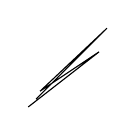
\begin{tikzpicture}\draw (0,0)--(.9,.7)--(.15,.2)--(1,1)--(.1,.1)--(.7,.7);\end{tikzpicture}}
\diagram{\begin{array}{c}
\Delta(1)\times X_{i+1}\\
\cup\\
(\Delta(1)\times X_i)\cup(\{0\}\times X_{i+1})\cup(\{1\}\times X_{\unsure{i-1|i+1}})
\end{array}}
\diagram{\begin{tikzcd}
Y\arrow[r,hook,-,shift right=.6pt]\arrow[r,<-,shift left=.6pt]&Z_0\arrow[r,hook,-]&Z_1\arrow[r,hook,-]&Z_2\mathbin{\cdots-}
\end{tikzcd}}
Assume $\forall i$, $\exists$ retraction $Z_i\mathbin{-}Y$

Is there a retraction $Z_\infty\longrightarrow Y$?

\uline{not clear at all}, \unsure{on|our} \deleted{\unsure{contrary}} the whole point is to see that
\[
\varprojlim_i\pi_0\underline{\operatorname{Retr}}(\unsure{Z_i|Z},Y)\ne\varnothing.\mathbin{-}
\]
Ask Ronnie Brown!
\mspage{24}
